\section{System Architecure}
\label{sec:systemarch}

This section presents the core elements of the Morpheus system and its 
role in the \textit{automated question answering} process. 

\subsection{Query Processing}
  
The \textit{Query Resolution Recorder} or QRR is an instrumented web browser
used to
track the search pathways to an answer for a \textit{guide user's} query. It
also facilitates guide user to identify output categories. All this information
is represented in an SSQ as described above. For example, suppose, a guide user
tries to answer the query "a 1997 Toyota Camry V6 needs what size tires?" using
Morpheus. With the help of QRR, he may choose relevant query terms and assign
categories to them: Toyota as the category manufacturer, Camry V6 as category
model, tire as the category automotive parts, and size as the output category
size. In addition, he can log the search pathways to an answer (e.g. P215/60R16)
to this query and select the query realm as automotive. Morpheus captures all
these information in the format of SSQ.     


The \textit{Query Resolution Method} or QRM is a data structure that models the
question answering process. A QRM is usually constructed by a guide user with
the help of the QRR. Each QRM contains an ontological realm, an SSQ, and
information to support the query answering process. QRMs are associated with an
ontology that
has a particular realm i.e. an ontological realm. The associated SSQ contains a
user query, selected terms and category associations, and output categories for
a given query. In addition, the QRM contains information required to visit each
page needed to answer the query as well as the order of visitation. For each
dyanamic page, it stores the list of inputs to the URL such as form inputs and
the possible referrence outputs (highlighted portions of the web page).


A \textit{regular} user query is parsed into specific terms by \textit{NLP
engine} using
some linguistic techniques [Need to be completed]. The SSQ generated by the NLP
Engine contains user query and parsed terms. 


\subsection{Morpheus Ontology and Corpora} 

Morpheus requires a realm-based ontology that contains categories of a
particular realm. For example, for the realm-ontology \textit{Automotive}
contains categories that are relevant to the \textit{automotive} realm. In
addition, every category in the ontology is associated with a corpus of words
that belongs to that category.   

For realm ontology construction Morpheus uses the Wikipedia pages, categories,
and the WordNet synset heterarchy. This approch is motivated from
YAGO\cite{Suchanek2009phd}. Morpheus creates a realm ontology as follows: For a
given realm, we first find a mapping category from the Wikipedia categories 
ontology. Then we grab all the neighboring categories
using a concept called a \textit{Markov Blanket} \cite{PRIS} in \textit{Bayesian
Networks}. In fact, we grab the category's parents, its children, and its 
children's other parents using the DBpedia ontology properties \textit{broader}
and \textit{narrower}. Once the blanket is ready, it grabs all parent categories
of the categories in the blanket till it reaches root. Once we have the
categories belongs to a particular domain, we associate them with WordNet synset
heterarchy using an algorithm similar to YAGO. We determine head noun in the
category name and search for it in the WordNet synsets\cite{Suchanek2009phd}.
Those Wikipedia categories having no WordNet match are ignored in the our realm
ontology.   

In order to build corpus for each of the categories in the ontology, 
we extract words from the Wikipedia pages those are associated with the 
the DBpedia categories \cite{Auer07dbpedia:a}. Every corpus is associated 
with corresponding category in the Morpheus ontology.  

\subsection{QRM Ranking Mechanism} 

To answer a regular user's queries that is in SSQ format (a \textit{candidate
SSQ}), Morpheus finds similar SSQs that belong to QRMs in the store (a
\textit{qualified SSQ}). We need a similarity measure to match the candidate SSQ
with a qualified SSQ within the Morpheus data store. For the SSQ similarity, we
consider the SSQ components [\ref{sec:morpheus}] such as query-realm, input
terms and output terms, and their assigned categories or classes. Thus,
\textit{category divergence}, a similarity measure, is defined for these classes
based on ontology's class heterarchy. It is motivated by the concept of multiple
dispatch in CLOS \cite{Steele1990} and Dylan programming \cite{Barrett1996} for
generic function type matches. Once we have the similarity measures between the
candidate SSQ and qualified SSQs in the QRM data store, we order the relevant
SSQs and associated QRMs. The order provides a ranking for the results to the
user. Subsections \ref{sec:ctd}, and \ref{sec:oqom} describe this in detail.

\subsubsection{Catgeory Divergence}
\label{sec:ctd}

We employ a measure of compatibility, which we call \textit{category
divergence},
between a source category and a target category using the \textit{topological
structure} of the categories in an ontology. We write $S \prec T$ for the
reflexive
transitive closure of the supercategory relation. Let $d(P,Q)$ represent the hop
distance in the directed ontology inheritance graph from $P$ to $Q$. The
divergence between a source and target category ranges from zero (for identical
categories) to one (for incompatible categories). Let $S$ be the source
category, $T$ be
the target category, and let $C$ be a least common ancestor category of $S$ and
$T$
minimizing $d(S,C) + d(T,C)$. The category divergence between $S$ and $T$ is
defined given by:

\begin{equation}
d_{cat}(S, T) = \begin{cases}
0 & S.{Uri} \equiv T.{Uri}\\
d(S, T)/(3h) & S \prec T\\
1 & T \prec S\\
(d(S,root) + d(S,C) \\ \ \ \ \ + d(T,C))/(3h) & otherwise
\end{cases}
\end{equation}

\noindent where $h$ is the height of the ontology tree.

Note, if $S \prec T$ and $S \not\prec Q$ then $d_{cat}(S,T) <
d_{cat}(S,Q)$, that is, the divergence of a source category to a target
ancestor category is smaller than the divergence of a source category to any
category that is not an ancestor. This is an important property in
determining the compatibility of category for answering queries.  If a
SSQ answers queries concerning an ancestor category, it is more relevant
that a SSQ that answers queries from any non-ancestral category.

% Algorithm 1: figure  
\begin{figure}[t]
\centering
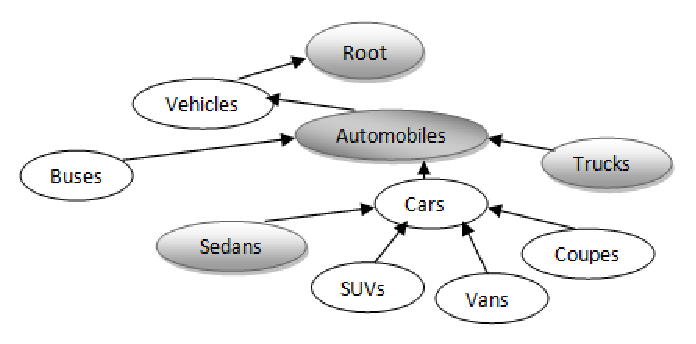
\includegraphics[width=90mm]{img/automotive_ontology.eps}
\caption{An abbreviated graphical representation of an automotive
ontology: This is a manually created ontology, from the Wikipedia category
hierarchy and pages. The edges represent inheritance relationships between the
category in a topology.}
\label{fig:automotive_ontology}
\end{figure}

Suppose we want to find the category divergence between \textit{Toyota Camry}
and \textit{Coupes} [Figure \ref{fig:automotive_ontology}]. 
\textit{Toyota Camry} is the subcategory of \textit{Sedans}, and \textit{Coupes}
is the subcategory of \textit{Cars}. Therefore, the least common ancestor ($C$)
for these two categories is \textit{Cars}. In addition, the tree height is $5$.
So, the normalized divergence $d_{cat}$\textit{(Toyota Camry, Coupes)} is $7/15$
that is calculated from \textit{d(Toyota Camry, Root)} is 5, \textit{d(Toyota
Camry, Cars)} is two, and \textit{d(Coupes, Cars)} is one.

\subsubsection{SSQ Ontology Matching}
\label{sec:oqom}

We use category divergence to calculate the relevance between the candiate SSQ
and a qualified SSQ associated with a QRM in the store. Each qualified SSQ will
have input terms, output terms, and associated classes, and one realm. For the
candidate SSQ, the relevant category for input terms are determined from the
ontology corpora. From a category term corpus, we can find out the likelihood
that a term belongs to a particular category. This is determined by the
probability of a category given a term using \textit{Bayes Rule} (Eq.
\ref{eq:bayesrule}), since we can easily obtain the term-category and
term-corpus probabilities as relative frequencies. The higher the probability,
the more likely a term is referring to a category. 

\begin{equation}
\label{eq:bayesrule}
P (category | term) = \frac{P(term | category) P(category)}{P(term)}
\end{equation}

The relevance of a qualified SSQ to the candidate SSQ is determined by
aggregating the divergence measure of categories associated with them. 

\subsection{Query Resolution Methods} 

Usually, answering a question using the 
deep web requires one to navigate through a sequence of one or 
more web pages. Many of the accesses involve clicks through 
web forms or links to resulting pages. QRM contains the necessary  
information required to re-run this procedure. Once we have 
relevant QRMs through QRM ranking for a given user query, we can  
get answers by re-running the pathways with help of QRE. 


  


